\documentclass[twoside,11pt]{article}
%\documentclass[UTF8]{ctexart}
\usepackage[heading=true]{ctex}

\usepackage{listings}
\usepackage{color}

\usepackage{subfig}

\usepackage{multirow}
\usepackage{booktabs}

\definecolor{dkgreen}{rgb}{0,0.6,0}
\definecolor{gray}{rgb}{0.5,0.5,0.5}
\definecolor{mauve}{rgb}{0.58,0,0.82}

\lstset{frame=tb,
  language=Python,
  aboveskip=3mm,
  belowskip=3mm,
  showstringspaces=false,
  columns=flexible,
  basicstyle={\small\ttfamily},
  numbers=none,
  numberstyle=\tiny\color{gray},
  keywordstyle=\color{blue},
  commentstyle=\color{dkgreen},
  stringstyle=\color{mauve},
  breaklines=true,
  breakatwhitespace=true,
  tabsize=3
}

\usepackage{fancyhdr} % 页眉页脚
\usepackage{graphicx}
\usepackage{amsmath}
\usepackage[colorlinks=true, allcolors=blue]{hyperref}
%\usepackage[margin=1.5in]{geometry}

\oddsidemargin .25in    %   Note \oddsidemargin = \evensidemargin
\evensidemargin .25in
\marginparwidth 0.07 true in
%\marginparwidth 0.75 true in
%\topmargin 0 true pt           % Nominal distance from top of page to top of
%\topmargin 0.125in
\topmargin -0.1in
\addtolength{\headsep}{0.25in}
\textheight 8.5 true in       % Height of text (including footnotes & figures)
\textwidth 6.0 true in        % Width of text line.
\widowpenalty=10000
\clubpenalty=10000


\pagestyle{fancy}

%\firstpageno{1}

\title{文本表征学习HW1}

\author{罗浩铭\ PB21030838}


\begin{document}

\fancyhf{} % 清除所有页眉页脚
\fancyfoot[C]{\thepage} % 设置右页脚为页码
\fancyhead[l]{\footnotesize USTC Text Representation Learning} % 设置左页眉为课程名称
% 设置右页眉为章节标题 

\renewcommand{\headrulewidth}{0pt} % 去页眉线

\begin{center}
  \textbf{\LARGE{文本表征学习HW1}}\\
  \vspace{0.1cm}
  \large{罗浩铭\ PB21030838}
\end{center}


% 实验报告要求:使用训练数据构建统计语言模型并使用不同平滑方法优化模型,对比分析不同模型及平滑策略在不同测试集上的性能(perplexity),完成并提交1-2页的实验报告


% ·bigram语言模型与trigram语言模型的比较分析
% ·通过语言模型在不使用平滑、使用加一平滑、使用古德-图灵平滑时在不同数据集上性能的比较,讨论比较不同平滑策略的优劣
% ·上述讨论与分析依据的具体模型参数和性能数值
% ·简要描述实现模型的过程,其中使用了哪些数据结构,遇到了哪些问题,是如何解决的


\section{模型实现}
\subsection{N-gram模型实现}
本次实验数据集中提供的句子均已完成分词,因此我们可以直接根据分词结果来构建N-gram模型。
我们读入每一行句子,并使用nltk.util.ngrams来生成每个句子中含有的n-gram序列(左右各填充"<bos>"与"<eos>"),将其合并为一个列表。
然后使用Python的collections.Counter类来统计每种n-gram出现的次数,作为频率。

则由此可以得到n-gram模型的概率估计,式中C即为上述频率:
\begin{equation}
  P(w_n|w_{n-1},w_{n-2},\cdots,w_1) = \frac{C(w_n,w_{n-1},w_{n-2},\cdots,w_1)}{C(w_{n-1},w_{n-2},\cdots,w_1)}
\end{equation}

\subsection{平滑方法实现}
本次实验中我们实现了两种平滑方法:加一平滑与Good-Turing平滑。
加一平滑的概率估计如下,式中V为单词表大小:
\begin{equation}
  P_{add1}(w_n|w_{n-1},w_{n-2},\cdots,w_1) = \frac{C(w_n,w_{n-1},w_{n-2},\cdots,w_1)+1}{C(w_{n-1},w_{n-2},\cdots,w_1)+V}
\end{equation}

Good-Turing平滑则通过对每个n元组的出现次数赋予一个新值$c^*$,将出现次数为c的n-gram频率映射到出现次数为c+1的n-gram的频率上,从而避免了出现次数为0的n-gram。
其中$c^*$由以下公式得到:
\begin{equation}
  c^* = \frac{(c+1)N(c+1)}{N(c)}
\end{equation}
而由于在实际应用中,$N(c+1)$可能为0,因此我们需要又对$N(c+1)$进行平滑处理,来避免出现除0错误。
这里我们使用了常见的Good-Turing平滑的实现方法,即对于出现次数为$c$的n元组个数$N_c$,采用线性拟合的方式得到:
\begin{equation}
  \log N_c = a + b \log c
\end{equation}
将拟合结果代入$c^*$的计算公式中,即可得到平滑后的频率。而对于出现次数为0的n元组,我们直接将其出现次数设为$N_1/N$。


\section{实验结果}
由于均值易受部分句子混乱度较极端影响,因此我们选择使用中位数作为性能指标。
\begin{table}[htbp]
  \renewcommand{\multirowsetup}{\centering}
  \caption{bigram与trigram模型在不同平滑方法下得到的Perplexity中位数}
  \label{tab:hyperparams}
  \vspace{5pt}
  \centering
  \begin{tabular}{cccc}
    \toprule
    \multicolumn{2}{c}{组别} & Bigram模型      & Trigram模型                               \\
    \midrule
    \multirow{3}{*}{测试集1} & 不使用平滑      & inf                 & inf                 \\
                             & 加一平滑        & $8.015 \times 10^3$ & $3.028 \times 10^4$ \\
                             & Good-Turing平滑 & $3.426 \times 10^2$ & $5.448 \times 10^1$ \\
    \midrule
    \multirow{3}{*}{测试集2} & 不使用平滑      & $7.230 \times 10^1$ & inf                 \\
                             & 加一平滑        & $2.056\times 10^3$  & $1.029 \times 10^4$ \\
                             & Good-Turing平滑 & $7.849 \times 10^1$ & $5.752 \times 10^1$ \\
    \bottomrule
  \end{tabular}
\end{table}

各组别下模型输出的Perplexity的对数的分布图如下:
% 下面是组图,横排3张
\begin{figure}[htbp]    % 常规操作\begin{figure}开头说明插入图片
  % 后面跟着的[htbp]是图片在文档中放置的位置,也称为浮动体的位置,关于这个我们后面的文章会聊聊,现在不管,照写就是了
  \centering            % 前面说过,图片放置在中间
  \subfloat[][无平滑]
  {
    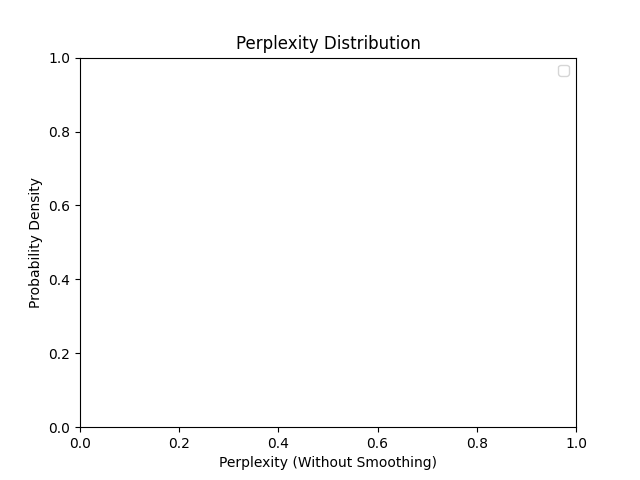
\includegraphics[width=0.3\textwidth]{./pic/perplexity_1_prob.png}    % 插入图片,[]中设置图片大小,{}中是图片文件名
  }
  \subfloat[][加一平滑]
  {
    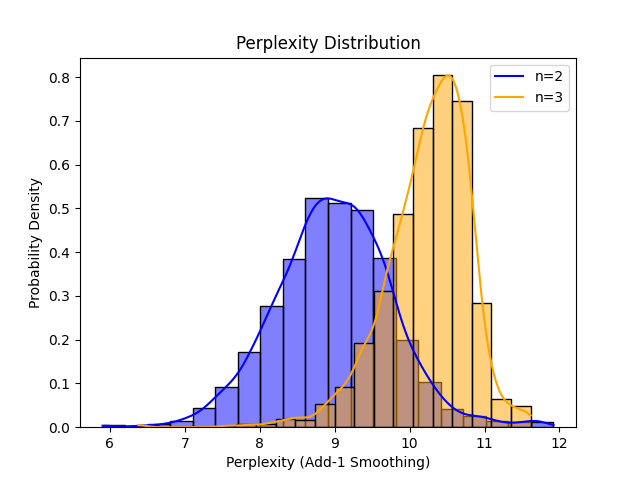
\includegraphics[width=0.3\textwidth]{./pic/perplexity_1_add_delta_prob.png}
  }
  \subfloat[][Good-Turing平滑]
  {
    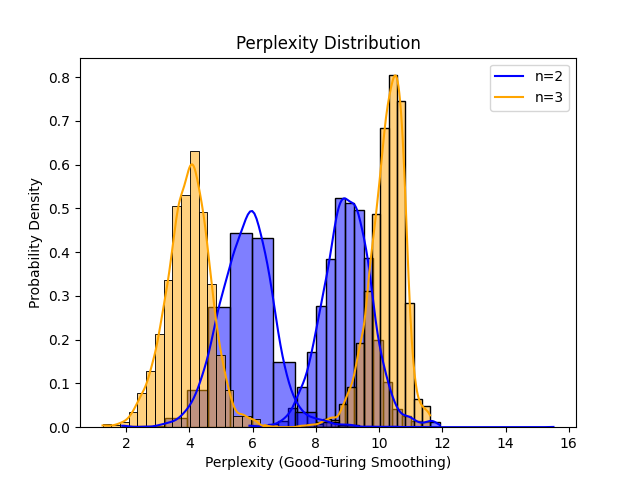
\includegraphics[width=0.3\textwidth]{./pic/perplexity_1_good_turing_prob.png}
  }
  \caption{测试集一中,不同平滑方法的Perplexity的对数分布图}    % 图的标题
  \label{fig:figs}    % 给图片一个标签,这样方便引用
\end{figure}

\begin{figure}[htbp]    % 常规操作\begin{figure}开头说明插入图片
  % 后面跟着的[htbp]是图片在文档中放置的位置,也称为浮动体的位置,关于这个我们后面的文章会聊聊,现在不管,照写就是了
  \centering            % 前面说过,图片放置在中间
  \subfloat[][无平滑]
  {
    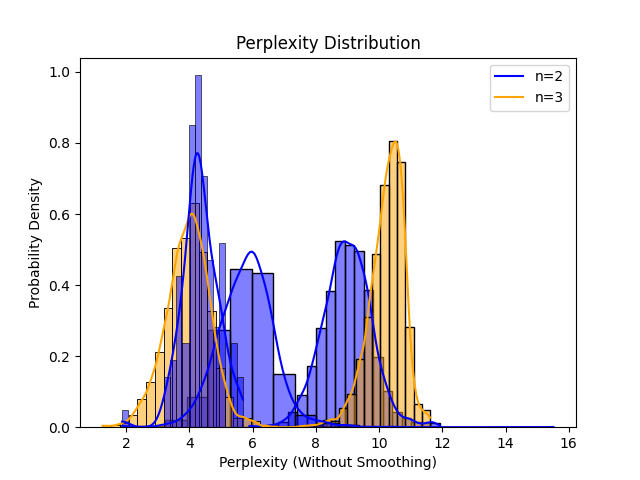
\includegraphics[width=0.3\textwidth]{./pic/perplexity_2_prob.png}    % 插入图片,[]中设置图片大小,{}中是图片文件名
  }
  \subfloat[][加一平滑]
  {
    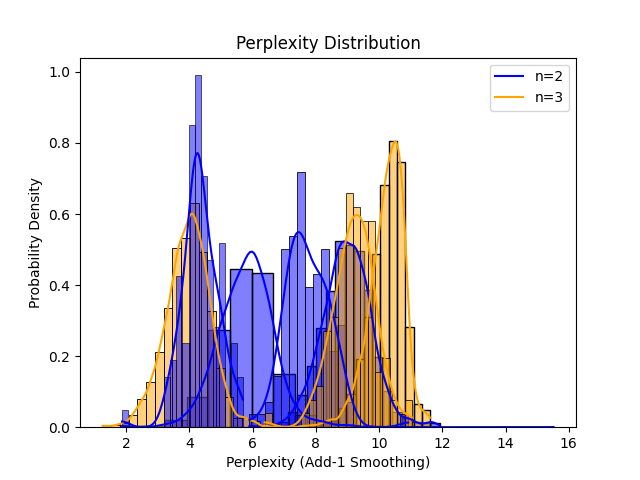
\includegraphics[width=0.3\textwidth]{./pic/perplexity_2_add_delta_prob.png}
  }
  \subfloat[][Good-Turing平滑]
  {
    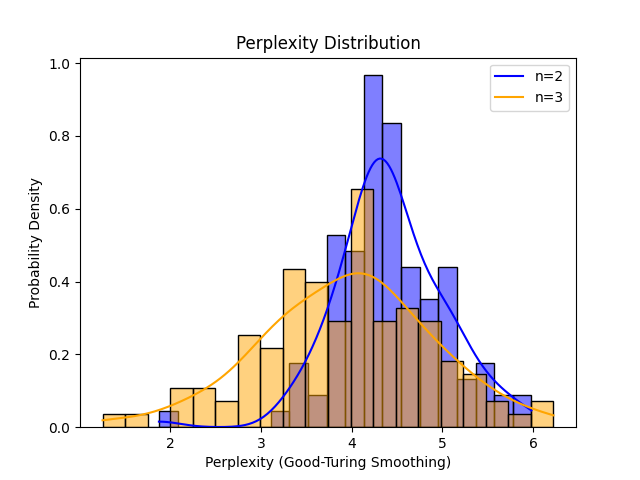
\includegraphics[width=0.3\textwidth]{./pic/perplexity_2_good_turing_prob.png}
  }
  \caption{测试集二中,不同平滑方法的Perplexity的对数分布图}    % 图的标题
  \label{fig:figs}    % 给图片一个标签,这样方便引用
\end{figure}


对比bigram模型与trigram模型的性能,我们可以看出:
\begin{itemize}
  \item 由于未使用平滑时,只有bigram模型在测试集2上取得了有效的结果(因其只有一个单词的上文,且测试集2不包含新词)。
  \item 在两个测试集上,当使用加一平滑时,bigram模型的性能要优于trigram模型,这可能是因为bigram参数空间小,训练得到的概率分布不那么平滑,不容易被加一平滑过度稀释。
  \item 在两个测试集上,当使用Good-Turing平滑时,trigram模型的性能要优于bigram模型,此时模型的表现符合预期。
  \item 此外,trigram模型预测的Perplexity通常更为两极分化。
\end{itemize}

对比不同平滑策略下的模型性能,可以发现:
\begin{itemize}
  \item 不使用平滑的情况下,由于部分n-gram未在训练集中出现,导致了Perplexity无穷大,则难以得到有效结果。
  \item 在各组别下,Good-Turing平滑的性能要远远优于加一平滑,这可能是因为加一平滑过度稀释了下一词预测的概率分布。
\end{itemize}

\end{document}

